% Cortex - Brussels North-South junction: five questions, Phase 0
% Build:  latexmk -pdf five_questions.tex     (or: pdflatex five_questions.tex x2)
% A lean, question-driven walkthrough of Phase 0. For the full lab notebook
% (data pipeline, SOTA survey, causal designs, reformulation narrative), see
% phase0_report.tex in this same directory.
\documentclass[aspectratio=169,10pt]{beamer}

\usepackage[utf8]{inputenc}
\usepackage[T1]{fontenc}
\usepackage{lmodern}
\usepackage{booktabs}
\usepackage{graphicx}
\usepackage{xcolor}
\usepackage{tikz}
\usetikzlibrary{arrows.meta, positioning}

\graphicspath{{figures/}{../../data/phase0/figures/}}

% ---- palette (matches the figures: validated categorical slots 1-3) ---------
\definecolor{surface}{HTML}{FCFCFB}
\definecolor{ink}{HTML}{0B0B0B}
\definecolor{ink2}{HTML}{52514E}
\definecolor{ink3}{HTML}{8A8880}
\definecolor{cblue}{HTML}{2A78D6}
\definecolor{corange}{HTML}{EB6834}
\definecolor{caqua}{HTML}{1BAF7A}
\definecolor{cgrid}{HTML}{E3E2DD}

\usetheme{default}
\usecolortheme{default}
\setbeamercolor{background canvas}{bg=surface}
\setbeamercolor{normal text}{fg=ink}
\setbeamercolor{frametitle}{fg=ink, bg=surface}
\setbeamercolor{structure}{fg=cblue}
\setbeamercolor{alerted text}{fg=corange}
\setbeamerfont{frametitle}{size=\large, series=\bfseries}
\setbeamertemplate{navigation symbols}{}
\setbeamertemplate{itemize items}[circle]
\setbeamertemplate{footline}{%
  \hfill\usebeamerfont{date}\color{ink3}\scriptsize\insertframenumber\hspace{2em}\vspace{1ex}}

\newcommand{\srcnote}[1]{{\scriptsize\color{ink3}#1}}
\newcommand{\hl}[1]{{\color{corange}\textbf{#1}}}
\newcommand{\qtag}[1]{{\scriptsize\color{surface}\colorbox{cblue}{\strut~Q#1~}}}

\title{\textbf{Delay at the Brussels North--South junction}}
\subtitle{Seven questions, Phase 0}
\author{TReC Causality Team}
\date{\today}

\begin{document}

\begin{frame}[plain]
  \titlepage
\end{frame}

% =============================================================== INTRO
\begin{frame}{The junction}
  The \textbf{Brussels North--South connection}: a six-track tunnel under central
  Brussels linking Bruxelles-Nord to Bruxelles-Midi, three intermediate stops.
  \textbf{Every train crossing Belgium north-to-south passes through it.}
  \hl{968 traversals per day.}

  \vspace{0.5em}
  \centering
  \resizebox{0.94\textwidth}{!}{%
  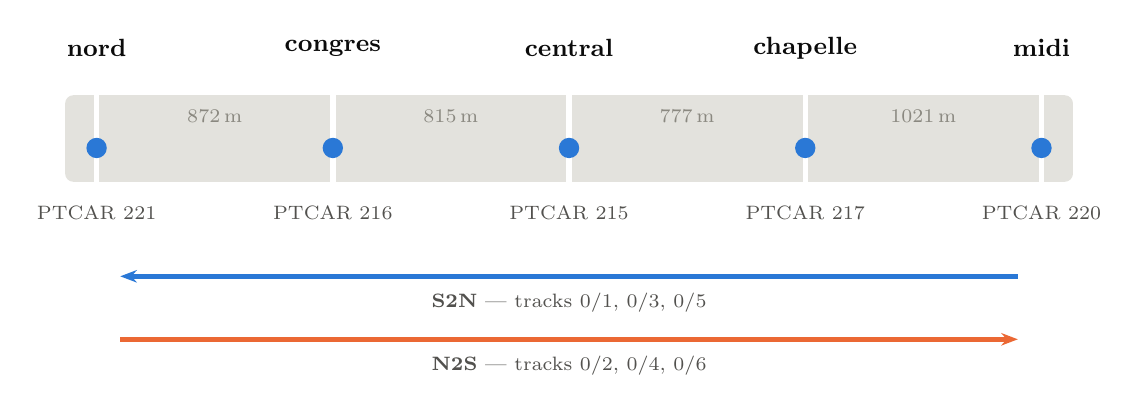
\begin{tikzpicture}[font=\small]
    \fill[cgrid, rounded corners=3pt] (-0.4,-0.55) rectangle (12.4,0.55);
    \foreach \a/\b/\d in {0/3/872, 3/6/815, 6/9/777, 9/12/1021}{
      \pgfmathsetmacro\mid{(\a+\b)/2}
      \node[font=\scriptsize, color=ink3] at (\mid,0.28) {\d\,m};
    }
    \foreach \x/\nm/\pt in {0/nord/221, 3/congres/216, 6/central/215, 9/chapelle/217, 12/midi/220}{
      \draw[white, line width=2pt] (\x,-0.55) -- (\x,0.55);
      \node[circle, fill=cblue, inner sep=2.6pt] at (\x,-0.12) {};
      \node[font=\small\bfseries, color=ink] at (\x,1.15) {\nm};
      \node[font=\scriptsize, color=ink2] at (\x,-0.95) {PTCAR \pt};
    }
    \draw[-{Stealth[length=6pt]}, cblue, line width=1.6pt] (11.7,-1.75) -- (0.3,-1.75);
    \node[font=\scriptsize, color=ink2] at (6,-2.08) {\textbf{S2N} --- tracks 0/1, 0/3, 0/5};
    \draw[-{Stealth[length=6pt]}, corange, line width=1.6pt] (0.3,-2.55) -- (11.7,-2.55);
    \node[font=\scriptsize, color=ink2] at (6,-2.88) {\textbf{N2S} --- tracks 0/2, 0/4, 0/6};
  \end{tikzpicture}}

  \vspace{0.6em}
  \raggedright\small
  Data: Infrabel open data, full year 2025, \textbf{338{,}914 traversals}. Each
  traversal is one train's crossing, with delay recorded at every point along the
  way.
\end{frame}

\begin{frame}{The objective, and why this deck is structured as seven questions}
  \textbf{Objective.} Use a SUMO microsimulation as an \hl{interventional ground
  truth} to validate causal-discovery methods for delay propagation, then apply the
  validated method to the real record.

  \vspace{0.6em}
  Before any of that, Phase 0 had to answer seven questions in order --- each one
  only makes sense once the previous one is settled:

  \vspace{0.4em}
  \begin{enumerate}
    \item \textbf{Does the delay distribution change} across the junction at all?
    \item \textbf{What is a chain} of delayed trains, and do they really happen?
    \item \textbf{Can we predict} how much delay a train gains? (regression)
    \item \textbf{Can we classify} whether a train will be meaningfully delayed?
    \item \textbf{Can we classify} whether a train will trigger a \emph{domino}?
    \item \textbf{Does delay skip a hop}, or is propagation strictly local?
    \item \textbf{Is ``station''} --- not just the train ahead --- a common cause?
  \end{enumerate}

  \vspace{0.7em}
  \begin{block}{\small The rule for every question}
    \small A number alone proves nothing. \textbf{Every answer below is measured
    against a baseline} --- a null hypothesis, an independence assumption, or a
    naive rule --- so the improvement, not just the score, is what gets reported.
  \end{block}
\end{frame}

% =============================================================== Q1
\begin{frame}{\qtag{1} Does the delay distribution change across the junction?}
  \textbf{Baseline / null hypothesis:} if the junction does nothing, the delay
  distribution \textbf{entering} should equal the delay distribution
  \textbf{leaving} --- same shape, same spread.

  \vspace{0.5em}
  \centering
  \begin{tabular}{@{}lrrr@{}}
    \toprule
    quantile & entering & leaving & shift \\
    \midrule
    5\% & $-6$\,s & $-37$\,s & $-31$ \\
    50\% & 34\,s & 63\,s & $+29$ \\
    90\% & 217\,s & 314\,s & $+97$ \\
    99\% & 585\,s & 730\,s & $+145$ \\
    \midrule
    \textbf{sd} & \textbf{141\,s} & \textbf{184\,s} & \textbf{+42} \\
    \bottomrule
  \end{tabular}
  \quad Cohen's $d=0.318$, KS $=0.148$

  \vspace{0.6em}
  \textbf{Answer: yes, the null is rejected}, but not the way it first looks.
  The typical (median) train's own change is tiny ($+6$\,s) --- yet the
  \emph{distribution} shifts \hl{+29\,s} at its median, because 54\% of trains lose
  time and 45\% gain, and the losses run almost twice the size of the gains.
  \srcnote{The junction disperses delay --- both tails stretch --- rather than
  adding a fixed amount to everyone.}
\end{frame}

\begin{frame}{\qtag{1} What the shift looks like}
  \centering
  \includegraphics[width=0.93\textwidth]{fig6_dispersion}

  \vspace{0.3em}
  \raggedright\small
  Early trains leave \emph{earlier}; late trains leave \emph{much} later.
  \hl{71.3\% of trains change by less than a minute either way} --- the 24.8\% that
  gain more than a minute account for essentially all the delay the junction adds.
  That concentration is why Questions 3--5 exist.
\end{frame}

% =============================================================== Q2
\begin{frame}{\qtag{2} What is a chain, and do they really happen?}
  \textbf{Definition.} Train $i$ links to train $i{-}1$ iff both were
  \emph{moved} (gained $>$60\,s) \emph{and} their headway is $\leq$5\,min, on the
  same track. A chain is a maximal run of linked trains.

  \vspace{0.4em}
  \textbf{Baseline / null hypothesis:} if trains were \textbf{independent}, knowing
  that one was moved would tell you nothing about the next one --- $P(\text{next
  moved}\mid\text{this moved}) = P(\text{next moved})$ unconditionally.

  \vspace{0.6em}
  \centering
  \begin{tabular}{@{}lrrr@{}}
    \toprule
    headway to next & P(next moved $\mid$ this moved) & P(next $\mid$ this NOT) & ratio \\
    \midrule
    $<$3 min & 92.1\% & 49.0\% & 1.9$\times$ \\
    3--5 min & 71.9\% & 14.6\% & \textbf{4.9$\times$} \\
    5--10 min & 28.5\% & 8.5\% & 3.4$\times$ \\
    $>$10 min & 14.0\% & 9.1\% & 1.5$\times$ \\
    \bottomrule
  \end{tabular}

  \vspace{0.6em}
  \textbf{Answer: independence is firmly rejected.} Of 89{,}463 moved events,
  \textbf{37.6\% chain to at least one more}; 63.2\% of all moved trains sit inside
  a chain of 2+; chains up to \textbf{18 trains} observed.
  \srcnote{Threshold checked from 15\,s to 300\,s: the chained share stays
  $\approx$58--60\% throughout --- not an artifact of the 60\,s cutoff.}
\end{frame}

% =============================================================== Q3
\begin{frame}{\qtag{3} Can we predict how much delay a train gains? (regression)}
  \textbf{Baselines:} \texttt{zero} (predict no change), \texttt{persistence}
  (exit delay $=$ entry delay --- the junction changes nothing), \texttt{mean-gain}
  (persistence plus the average gain).

  \vspace{0.3em}
  \srcnote{\textbf{GBDT features:} own entry delay, hour, tunnel track, direction,
  service \srcnote{(base)} $+$ headway to leader, leader's entry delay
  \srcnote{(interaction block)}.}

  \vspace{0.4em}
  \centering
  \begin{tabular}{@{}lrr@{}}
    \toprule
    model & MAE & RMSE \\
    \midrule
    zero & 171.4\,s & 380.3\,s \\
    \textbf{persistence} & \textbf{60.2\,s} & \textbf{99.4\,s} \\
    mean-gain & 63.1\,s & 94.1\,s \\
    GBDT, no interaction features & 66.1\,s & 143.2\,s \\
    GBDT, + headway/leader state & 57.4\,s & 127.1\,s \\
    \bottomrule
  \end{tabular}

  \vspace{0.3em}

  \srcnote{The no-interaction row loses to persistence on both columns.}

  \vspace{0.6em}
  \textbf{Answer: marginal, and fragile.} Full-year rolling origin (9 folds): mean
  $+4.0\%$ MAE over persistence, \textbf{wins in 8 of 9 months, loses in July}; RMSE
  is \hl{worse in every single fold}. Regression is not the question this data
  answers well --- see Q1: most of the target is 71\% noise around zero.
\end{frame}

% =============================================================== Q4
\begin{frame}{\qtag{4} Can we classify whether a train will be meaningfully delayed?}
  \textbf{Target:} gain $>$60\,s (base rate 25.1\%).
  \textbf{Baseline:} the trivial rule ``headway $<$5\,min $\Rightarrow$ at risk''.

  \vspace{0.3em}
  \srcnote{\textbf{GBDT features:} headway to leader, leader's entry delay, own
  entry delay, hour, month, tunnel track, direction, service, temperature, rain,
  snowfall.}

  \vspace{0.4em}
  \centering
  \begin{tabular}{@{}lrrr@{}}
    \toprule
    model & ROC AUC & PR AUC & lift @ top 10\% \\
    \midrule
    trivial rule (headway $<$5 min) & 0.692 & 0.371 & 1.71$\times$ \\
    \textbf{GBDT, all features} & \textbf{0.811} & \textbf{0.639} & \textbf{3.08$\times$} \\
    \bottomrule
  \end{tabular}

  \vspace{0.3em}
  \srcnote{At the stricter 120\,s threshold: 0.703 $\to$ \textbf{0.828}, lift 3.93$\times$.}

  \vspace{0.5em}
  \raggedright
  \textbf{Answer: a clear, stable win.} Tested on 3 held-out months never seen in
  training. Calibration is honest too: predicted risk 0.04--0.81, actual
  0.05--0.77. \hl{Reformulating the target from ``how many seconds'' to ``will it
  cross a threshold'' is what makes the signal usable} --- same features, same
  data, a much better-posed question.
\end{frame}

% =============================================================== Q5
\begin{frame}{\qtag{5} Can we classify whether a train will trigger a domino?}
  \textbf{Target:} at the moment train $i$ exits, will the \emph{next} train on the
  same track also be moved? \textbf{Baseline:} the naive rule ``I'm late, so is
  whoever's next''.

  \vspace{0.3em}
  \srcnote{\textbf{GBDT features:} this train's own moved status and exit delay,
  gap to the next train \srcnote{(actual or scheduled --- see below)}, hour,
  month, tunnel track, direction, service, temperature, rain, snowfall.}

  \vspace{0.4em}
  \centering
  \begin{tabular}{@{}lrrr@{}}
    \toprule
    model & ROC AUC & PR AUC & lift @ top 10\% \\
    \midrule
    naive: ``I'm late, so is next'' & 0.689 & 0.397 & --- \\
    retrospective GBDT \srcnote{(uses actual next-gap)} & 0.864 & 0.777 & 3.69$\times$ \\
    \textbf{operational GBDT} \srcnote{(uses only the \emph{scheduled} next-gap)} & \textbf{0.859} & 0.738 & \textbf{3.47$\times$} \\
    \bottomrule
  \end{tabular}

  \vspace{0.6em}
  \textbf{Answer: the strongest predictive result in this deck}, and the only one
  directly deployable as a real-time alert --- the operational version needs only
  the timetable and the current train's own state. \srcnote{Checked that this is
  not just autocorrelation: even a train that is currently \emph{on time} still
  scores AUC 0.787 from headway and context alone.}
\end{frame}

\begin{frame}{Features used in each model}
  All models: gradient-boosted trees (\texttt{HistGradientBoostingClassifier} /
  \texttt{Regressor}), trained on months 1--9, tested on 10--12, held out.
  \hl{Every feature is knowable at the prediction moment} --- entry to the junction
  (Q3, Q4) or exit (Q5). No feature ever looks into the future.

  \vspace{0.5em}
  \centering\small
  \begin{tabular}{@{}p{2.1cm}p{4.0cm}p{4.0cm}p{2.4cm}@{}}
    \toprule
    & Q3 regression & Q4 classify moved & Q5 domino \\
    \midrule
    own state & entry delay & entry delay & moved status, exit delay \\
    neighbour & headway, leader's entry delay & headway, leader's entry delay &
      gap to \emph{next} train \\
    context & hour, track, direction, service & hour, month, track, direction,
      service & hour, month, track, direction, service \\
    weather & --- & temperature, rain, snowfall & temperature, rain, snowfall \\
    \bottomrule
  \end{tabular}

  \vspace{0.8em}
  \raggedright
  \srcnote{Q5's ``gap to next train'' comes in two versions: \textbf{actual} (only
  knowable once that train has departed --- retrospective) and \textbf{scheduled}
  (known from the timetable in advance --- operational, the deployable one).}

  \vspace{0.4em}
  By permutation importance (Q4 model): \hl{headway dominates} (AUC drop 0.172),
  then hour (0.062), track (0.020), leader's delay (0.019), own delay (0.013).
  Weather contributes $\approx$0 in every model tested.
\end{frame}

% =============================================================== Q6
\begin{frame}{\qtag{6} Does delay skip a hop, or is propagation strictly local?}
  \textbf{Setup.} For chains of length $\geq$3 (A $\to$ B $\to$ C, same track,
  linked as in Q2): does A (two hops back) still predict C's exit delay once B's
  \emph{full} state is controlled for?

  \vspace{0.4em}
  \textbf{Baseline / null hypothesis:} if propagation is \textbf{strictly local}
  (pure relay --- each train only reacts to whoever is immediately ahead), then
  controlling for B should fully explain away A's association with C. The
  partial correlation should collapse to $\approx$0.

  \vspace{0.6em}
  \centering
  \begin{tabular}{@{}lr@{}}
    \toprule
    quantity & value \\
    \midrule
    raw $r$(A's exit delay, C's exit delay) & $+0.359$ \\
    partial $r$ $\mid$ B's exit/entry delay, both headways, hour, month & $+0.228$ \\
    \bottomrule
  \end{tabular}

  \vspace{0.3em}
  \srcnote{$n=8{,}836$ chains of length $\geq$3.}

  \vspace{0.4em}
  \textbf{Answer: no --- the null is rejected.} \hl{63\% of the raw association
  survives} controlling for B. Not pure first-order relay: the chain's
  \emph{starter} still matters two hops downstream, beyond what its immediate
  neighbor explains. That residual is what Question 7 goes looking for.
\end{frame}

% =============================================================== Q7
\begin{frame}{\qtag{7} Is ``station'' --- not just the train ahead --- a common cause?}
  \textbf{Setup.} Two trains on \emph{different} tracks cannot physically queue
  behind each other. Compare same-track vs.\ cross-track correlation of delay
  \textbf{at Central} (the identified bottleneck), \textbf{matched on time-gap}
  so proximity cannot confound the comparison.

  \vspace{0.4em}
  \textbf{Baseline / null hypothesis:} if propagation is \textbf{purely
  track-specific} (relay/queueing only), cross-track correlation should collapse
  toward independence at every time-gap, since there is no physical mechanism
  linking two different tracks.

  \vspace{0.5em}
  \centering
  \begin{tabular}{@{}lrrrr@{}}
    \toprule
    time gap & same-track $r$ & $n$ & cross-track $r$ & $n$ \\
    \midrule
    60--120s & 0.373 & 1{,}166 & 0.131 & 490{,}848 \\
    180--300s & 0.419 & 289{,}060 & 0.124 & 962{,}672 \\
    450--600s & 0.303 & 270{,}518 & 0.138 & 1{,}227{,}524 \\
    \bottomrule
  \end{tabular}

  \vspace{0.6em}
  \textbf{Answer: the null is rejected too --- both mechanisms are real.}
  Cross-track correlation is \hl{flat at $\approx$0.13 across every distance}
  (station-wide ambient congestion, not decaying with proximity) --- \emph{but}
  same-track is \textbf{2--4$\times$ higher} at every matched gap. Station
  congestion is a genuine common cause, and it explains part of Q6's residual ---
  but it does not explain it away: sharing a track still adds a large,
  independent effect on top.
\end{frame}

% =============================================================== SUMMARY
\begin{frame}{The seven answers, together}
  \centering\small
  \begin{tabular}{@{}p{0.6cm}p{4.6cm}p{3.4cm}p{2.7cm}@{}}
    \toprule
    & question & baseline & result \\
    \midrule
    Q1 & does the distribution change? & no-change null & \textbf{yes} --- disperses \\
    Q2 & what is a chain? & independence & \textbf{37.6\% chain} \\
    Q3 & predict seconds gained? & persistence & \hl{marginal, fragile} \\
    Q4 & classify ``meaningfully delayed''? & headway rule & \textbf{AUC 0.81} \\
    Q5 & classify ``triggers a domino''? & naive propagation & \textbf{AUC 0.86} \\
    Q6 & does delay skip a hop? & full mediation & \textbf{63\% survives} \\
    Q7 & is station a common cause? & pure track relay & \textbf{both real} \\
    \bottomrule
  \end{tabular}

  \vspace{1em}
  \raggedright
  \begin{block}{\small The pattern across all seven}
    \small The sharper and more concentrated the question, the more the model beats
    its baseline. \textbf{Regression on the whole population is weak}
    because most of the population barely moves (Q1). \textbf{Classification on the
    affected minority is strong} (Q4), and \textbf{classification of propagation is
    strongest of all} (Q5) --- because that is where the causal mechanism lives.
    \textbf{Q6--Q7 open that mechanism up}: propagation is not a simple relay ---
    it is a mix of local track queueing and ambient station-wide congestion,
    \hl{both genuine, both quantified, neither explaining the other away}.
  \end{block}
\end{frame}

\end{document}
